\section{The Work: CHANGE ME -- might be 'Visual Design' or 'Experimental
Design'} % or "Research Plan"
\label{sec:vis}

Describe what you have done here. You may want to break this up into multiple
sections. If you are doing a design study, describe the methodology leading to
your design, not just the design itself.

Describe your proposed work here. You may refer to other sections so as not to
repeat yourself -- for example, referencing Section~\ref{sec:background}.

You may want to use figures to illustrate your point, such as
Figure~\ref{fig:sample}.

\begin{figure}[h]
 \centering % avoid the use of \begin{center}...\end{center} and use \centering instead (more compact)
 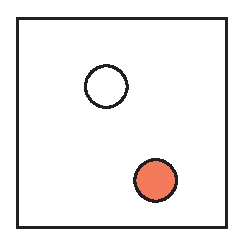
\includegraphics[width=\columnwidth]{figs/sample} 
 \caption{Figure illustrating some component of your design.}
 \label{fig:sample}
\end{figure}

%\begin{figure*}[h]
% \centering 
% 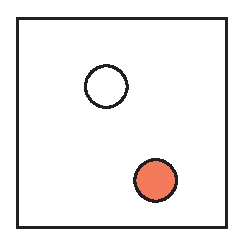
\includegraphics[width=\textwidth]{figs/sample} 
% \caption{Double Column Figure.}
% \label{fig:sample2}
%\end{figure*}

